\documentclass[thesis.tex]{subfiles}

\begin{document}


\begin{align}
  \hat{H} = H_\varnothing + \sum_{p q} H_{p q} \normord{\hat{a}_p^\dagger \hat{a}_q^{}} + \frac{1}{4} \sum_{p q r s} H_{p q r s} \normord{\hat{a}_p^\dagger \hat{a}_q^\dagger \hat{a}_s^{} \hat{a}_r^{}},
  \label{eq:normordhamiltonian}
\end{align}


Particle attached and particle removed equations-of-motion (EOM) methods can be coupled with either IM-SRG or CC calculations. The principal idea is that one may construct a ladder operator $\hat{X}$ that promotes the $N$-particle ground state to any state in the $N + 1$ or $N - 1$ spectrum,
\begin{equation}\label{eq:ladder_def}
  \ket{\Psi^{(N \pm 1)}_u}  = \hat{X}^{(N \pm 1)}_u \ket{\Psi^{(N)}_0},
\end{equation}
where $\hat{X}$ is in principle a linear combination of excitation $(+)$ and de-excitation $(-)$ operators that change particle number by one,
\begin{align}
  \label{eq:gen_attached}
  \hat{X}^{(N + 1)}_u &= \sum_a x^{(u, +)}_a  \normord{\hat{a}^\dagger_a} + \frac{1}{2} \sum_{a b i} x^{(u, +)}_{a b i} \normord{\hat{a}^\dagger_a \hat{a}^\dagger_b \hat{a}_i^{}} + \cdots,  \\
  \label{eq:gen_removed}
  \hat{X}^{(N - 1)}_u &= \sum_i x_i^{(u, -)} \normord{\hat{a}_i^{}} + \frac{1}{2} \sum_{i j a} x^{(u, -)}_{a i j} \normord{\hat{a}^\dagger_a \hat{a}_j^{} \hat{a}_i^{}}  + \cdots.
\end{align}
Here, $x^{(u, \pm)}_p$ and $x^{(u, \pm)}_{p q r}$ are the normal-ordered matrix elements of $\hat{X}_u^{(N \pm 1)}$, defined analogously to Eq.\ \eqref{eq:normordhamiltonian}.

Substitution of Eq.\ \eqref{eq:ladder_def} into the energy eigenvalue problem
\begin{gather*}
  \hat H \ket{\Psi_u^{(N \pm 1)}} = E^{(N\pm1)}_u \ket{\Psi_u^{(N \pm 1)}},
\end{gather*}
gives
\begin{equation}\label{eq:EOM}
  [\hat{H}, \hat{X}^{(N \pm 1)}_u] \ket{\Psi^{(N)}_0} = \pm \varepsilon^{(\pm)}_u \hat{X}^{(N \pm 1)}_u \ket{\Psi^{(N)}_0},
\end{equation}
which constitutes a generalized eigenvalue problem for the amplitudes $x$, where $\varepsilon^{(\pm)}_u$ are the single-particle addition ($+$) and removal ($-$) energies. The quality of this calculation depends on the ansatz for the $N$-particle ground state, as well as the systematically improvable truncation on the ladder operators. In this work we include 1p and 2p1h excitations in the $N + 1$ ladder operator and likewise 1h and 2h1p operators for the $N - 1$ ladder operators.

After a single-reference ground state IM-SRG calculation, the Hamiltonian has been rotated such that the reference state is an eigenfunction with corresponding eigenvalue $E^{(N)}_0$, which is the correlated $N$-particle ground state energy. The EOM equation is therefore
\begin{align} \label{eq:EOMIMSRG}
  [\bar{H},\bar{X}^{(N \pm 1)}_u] \ket{\Phi^{(N)}_0} = \pm \varepsilon^{(\pm)}_u \bar{X}^{(N \pm 1)}_u \ket{\Phi^{(N)}_0},
\end{align}
where bars denote rotated operators. Now the reference state is used in place of the bare correlated ground state. The ground state IM-SRG procedure has implicitly re-summed contributions from higher order excitations (3-particle-2-hole, 2-particle-3-hole, 2-particle-3-hole, 4-particle-3-hole, \ldots) into the lower order amplitudes of the ladder operators (1-particle-0-hole, 0-particle-1-hole, 2-particle-1-hole, 1-particle-2-hole).

Despite these gains, the EOM calculation is still a partial diagonalization method, limited by the truncation to 2-particle-1-hole and 1-particle-2-hole operators. We expect $N + 1$ (or $N - 1$) states to be described appropriately by EOM-IM-SRG if their wavefunctions are dominated by 1-particle-0-hole (or 0-particle-1-hole) contributions in the rotated frame. We use partial norms of the EOM ladder operators to estimate these contributions:
\begin{align}
  \label{eq:partial_norms_p}
  n_{\text{1-particle}} &= \sqrt{\sum_a | \bar{x}^{(+)}_a |^2},\\
  \label{eq:partial_norms_h}
  n_{\text{1-hole}} &= \sqrt{\sum_i | \bar{x}^{(-)}_i |^2}.
\end{align}
Large single particle partial norms indicate that the EOM truncation is reasonable for the relevant state. States with lower single particle norms should be treated with a higher EOM approximation, which can be accomplished directly or perturbatively \cite{PARZUCHOWSKI2017044304}.

Like EOM-IM-SRG, the equations-of-motion technique can be applied after a CC ground-state calculation, by using the CC effective Hamiltonian.  Here, the non-Hermitian nature of $\bar{H}_{\mathrm{CC}}$ becomes apparent.  In this case, in addition to constructing excitation ladder operators Eq.\ \eqref{eq:gen_attached} and Eq.\ \eqref{eq:gen_removed} that correspond to the right-eigenvectors of the generalized eigenvalue problem Eq.\ \eqref{eq:EOMIMSRG}, there exist analogous de-excitation ladder operators, $\hat{L}^{(N + 1)}$ and $\hat{L}^{(N - 1)}$, that correspond to the left-eigenvectors,
\begin{align*}
    \hat{L}^{(N + 1)}_u &= \sum_a l^{(u, +)}_a \normord{\hat{a}_a^{}} + \frac{1}{2} \sum_{i a b} l^{(u, +)}_{i a b} \normord{\hat{a}^\dagger_i \hat{a}_b^{} \hat{a}_a^{}} + \cdots, \\
    \hat{L}^{(N - 1)}_u &= \sum_i l_i^{(u, -)} \normord{\hat{a}^\dagger_i} + \frac{1}{2} \sum_{i j a} l^{(u, -)}_{i j a} \normord{\hat{a}^\dagger_i \hat{a}^\dagger_j \hat{a}_a^{}} + \cdots,
\end{align*}
where $l^{(u, \pm)}_p$ and $l^{(u, \pm)}_{p q r}$ are likewise the normal-ordered matrix elements of $\hat{L}^{(N \pm 1)}_u$.  These left-eigenvectors satisfy the left-eigenvalue problem, with left-eigenvalues $\varepsilon^{(\pm)}_u$, analogous to Eq.\ \eqref{eq:EOMIMSRG},
\begin{align*}
  \bra{\Phi^{(N)}_0} [\bar{H}, \bar{L}^{(N \pm 1)}_u] = \pm \varepsilon^{(\pm)}_u \bra{\Phi^{(N)}_0} \bar{L}^{(N \pm 1)}_u
\end{align*}
and form a bi-orthogonal set with the right-eigenvectors, $\braket{\bar{L}^{(N \pm 1)}_u}{\bar{X}^{(N \pm 1)}_v} = \delta_{u v}$.

In this paper, because the effective Hamiltonian is real, the corresponding left- and right-eigenvalues are equal. In addition, while the the left- and right-eigenvectors are generally not equivalent, the differences in their single-particle Eq.\ \eqref{eq:partial_norms_p} or single-hole Eq.\ \eqref{eq:partial_norms_h} natures are, in practice, not significant.  Therefore, only the right-eigenvectors are used in this paper.


%\begin{align}
%  \langle\Phi_{0}|\hat{L}^{+1}_{\nu}\bar{H}_{N}\hat{R}^{+1}_{\nu}|\Phi_{0}\rangle_{c} &= \diagram{PA_EOM/PA_EOM-figure0} + \diagram{PA_EOM/PA_EOM-figure1} + \diagram{PA_EOM/PA_EOM-figure2} + \diagram{PA_EOM/PA_EOM-figure3} \notag \\
%  &\hspace{-2cm} + \diagram{PA_EOM/PA_EOM-figure4} + \diagram{PA_EOM/PA_EOM-figure5} + \diagram{PA_EOM/PA_EOM-figure6} + \diagram{PA_EOM/PA_EOM-figure7} \notag \\
%\end{align}

%\begin{align}
%  \langle\Phi_{0}|\hat{L}^{-1}_{\nu}\bar{H}_{N}\hat{R}^{-1}_{\nu}|\Phi_{0}\rangle_{c}\ &= \diagram{PR_EOM/PR_EOM-figure0} + \diagram{PR_EOM/PR_EOM-figure1} + \diagram{PR_EOM/PR_EOM-figure2} + \diagram{PR_EOM/PR_EOM-figure3} \notag \\
%  &\hspace{-2cm} + \diagram{PR_EOM/PR_EOM-figure4} + \diagram{PR_EOM/PR_EOM-figure5} + \diagram{PR_EOM/PR_EOM-figure6} + \diagram{PR_EOM/PR_EOM-figure7} \notag \\
%\end{align}



\begin{align}
  \diagram{PA_EOM1/PA_EOM1-figure0} &= \diagram{PA_EOM1/PA_EOM1-figure1} + \diagram{PA_EOM1/PA_EOM1-figure2} + \diagram{PA_EOM1/PA_EOM1-figure3} \notag \\
  \omega_{k}\rop{a}{} &= \sum\limits_{c}\xint{a}{c}\rop{c}{} + \sum\limits_{kc}\xint{k}{c}\rop{ac}{k} + \frac{1}{2}\sum\limits_{kcd}\xint{ak}{cd}\rop{cd}{k}
\end{align}
\begin{align}
  \diagram{PA_EOM1/PA_EOM1-figure4} &= \diagram{PA_EOM1/PA_EOM1-figure5} + \diagram{PA_EOM1/PA_EOM1-figure6} + \diagram{PA_EOM1/PA_EOM1-figure7} + \diagram{PA_EOM1/PA_EOM1-figure8} \notag \\
  &+ \diagram{PA_EOM1/PA_EOM1-figure9} + \diagram{PA_EOM1/PA_EOM1-figure10} \notag \\
  \omega_{k}\rop{ab}{i} &= \sum\limits_{c}\xint{ab}{ci}\rop{c}{} + \Perm{ab}\sum\limits_{c}\xint{b}{c}\rop{ac}{i} - \sum\limits_{k}\xint{k}{i}\rop{ab}{k} + \frac{1}{2}\sum\limits_{cd}\xint{ab}{cd}\rop{cd}{i} \notag \\
  &-\Perm{ab}\sum\limits_{kc}\xint{ak}{ci}\rop{cb}{k} - \frac{1}{2}\sum\limits_{klcd}\vint{kl}{cd}\amp{ab}{ki}\rop{cd}{l}
\end{align}

\begin{align}
  \diagram{PA_EOM1/PA_EOM1-figure11} &= \diagram{PA_EOM1/PA_EOM1-figure12} + \diagram{PA_EOM1/PA_EOM1-figure13} \notag \\
  E_{k}\lop{}{a} &= \sum\limits_{c}\lop{}{c}\xint{c}{a} + \frac{1}{2}\sum\limits_{kcd}\lop{k}{cd}\xint{cd}{ak}
\end{align}
\begin{align}
  \diagram{PA_EOM1/PA_EOM1-figure14} &= \diagram{PA_EOM1/PA_EOM1-figure15} + \diagram{PA_EOM1/PA_EOM1-figure16} + \diagram{PA_EOM1/PA_EOM1-figure17} + \diagram{PA_EOM1/PA_EOM1-figure18} \notag \\
  &+ \diagram{PA_EOM1/PA_EOM1-figure19} + \diagram{PA_EOM1/PA_EOM1-figure20} + \diagram{PA_EOM1/PA_EOM1-figure21} \notag \\
  E_{k}\lop{i}{ab} &= \Perm{ab}\lop{}{a}\xint{i}{b} + \sum\limits_{c}\lop{}{c}\xint{ci}{ab} - \sum\limits_{k}\lop{k}{ab}\xint{i}{k} + \Perm{ab}\sum\limits_{c}\lop{i}{ac}\xint{c}{b} \notag \\
  &+ \frac{1}{2}\sum\limits_{cd}\lop{i}{cd}\xint{cd}{ab} - \Perm{ab}\sum\limits_{kc}\lop{k}{cb}\xint{ci}{ak} - \frac{1}{2}\sum\limits_{klcd}\lop{l}{cd}\vint{ki}{ab}\amp{cd}{kl}
\end{align}


\begin{align}
  \diagram{PR_EOM1/PR_EOM1-figure0} &= \diagram{PR_EOM1/PR_EOM1-figure1} + \diagram{PR_EOM1/PR_EOM1-figure2} + \diagram{PR_EOM1/PR_EOM1-figure3} \notag \\
  \omega_{k}\rop{}{i} &= -\sum\limits_{k}\xint{k}{i}\rop{}{k} + \sum\limits_{kc}\xint{k}{c}\rop{c}{ik} - \frac{1}{2}\sum\limits_{klc}\xint{kl}{ic}\rop{c}{kl}
\end{align}
\begin{align}
  \diagram{PR_EOM1/PR_EOM1-figure4} &= \diagram{PR_EOM1/PR_EOM1-figure5} + \diagram{PR_EOM1/PR_EOM1-figure6} + \diagram{PR_EOM1/PR_EOM1-figure7} + \diagram{PR_EOM1/PR_EOM1-figure8} \notag \\
  &+ \diagram{PR_EOM1/PR_EOM1-figure9} + \diagram{PR_EOM1/PR_EOM1-figure10} \notag \\
  \omega_{k}\rop{a}{ij} &= -\sum\limits_{k}\xint{ka}{ij}\rop{}{k} - \Perm{ij}\sum\limits_{k}\xint{k}{j}\rop{a}{ik} + \sum\limits_{c}\xint{a}{c}\rop{c}{ij} + \frac{1}{2}\sum\limits_{kl}\xint{kl}{ij}\rop{a}{kl} \notag \\
  &-\Perm{ij}\sum\limits_{kc}\xint{ak}{ci}\rop{c}{kj} - \frac{1}{2}\sum\limits_{klcd}\vint{kl}{cd}\amp{ca}{ij}\rop{d}{kl}
\end{align}

\begin{align}
  \diagram{PR_EOM1/PR_EOM1-figure11} &= \diagram{PR_EOM1/PR_EOM1-figure12} + \diagram{PR_EOM1/PR_EOM1-figure13} \notag \\
  E_{k}\lop{i}{} &= -\sum\limits_{k}\lop{k}{}\xint{i}{k} - \frac{1}{2}\sum\limits_{klc}\lop{kl}{c}\xint{ic}{kl}
\end{align}
\begin{align}
  \diagram{PR_EOM1/PR_EOM1-figure14} &= \diagram{PR_EOM1/PR_EOM1-figure15} + \diagram{PR_EOM1/PR_EOM1-figure16} + \diagram{PR_EOM1/PR_EOM1-figure17} + \diagram{PR_EOM1/PR_EOM1-figure18} \notag \\
  &+ \diagram{PR_EOM1/PR_EOM1-figure19} + \diagram{PR_EOM1/PR_EOM1-figure20} + \diagram{PR_EOM1/PR_EOM1-figure21} \notag \\
  E_{k}\lop{ij}{a} &= \Perm{ij}\lop{i}{}\xint{j}{a} - \sum\limits_{k}\lop{k}{}\xint{ij}{ka} + \sum\limits_{c}\lop{ij}{c}\xint{c}{a} - \Perm{ij}\sum\limits_{k}\lop{ik}{a}\xint{j}{k} \notag \\
  &+ \frac{1}{2}\sum\limits_{cd}\lop{kl}{a}\xint{ij}{kl} - \Perm{ij}\sum\limits_{kc}\lop{kj}{c}\xint{ci}{ak} - \frac{1}{2}\sum\limits_{klcd}\lop{kl}{d}\vint{ij}{ca}\amp{cd}{kl}
\end{align}

\begin{figure}[h]
  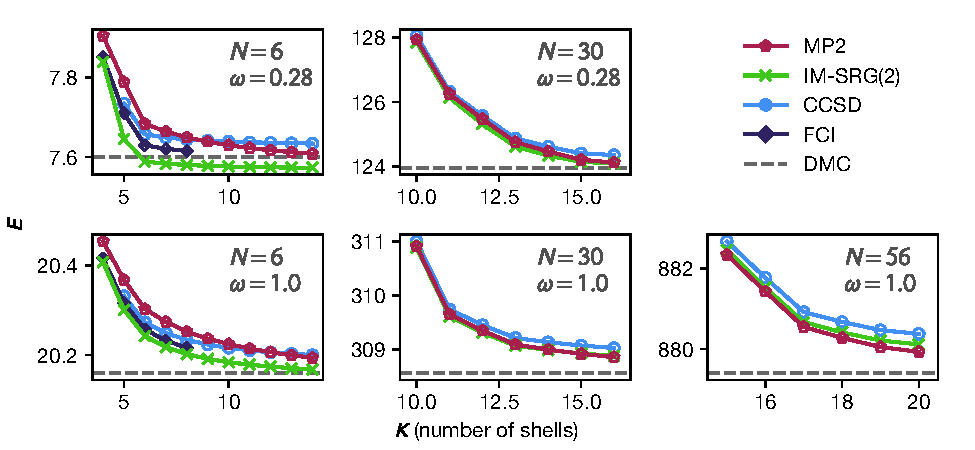
\includegraphics[width=\linewidth]{EOM/fig-gs2.pdf}
  \caption{CCD energy per electron in Hartrees for the 3D homogeneous electron gas as function of the Wigner-Seitz radius in units of Bohr radii. The calculation used periodic boundary conditions and a basis with 25 shells, resulting in a total of $1238$ single-particle states. Also plotted are the variational quantum Monte Carlo (QMC) results from \cite{LOPEZ2006}.}
  \label{fig:QDground}
\end{figure}

\begin{figure}[h]
  \centering
  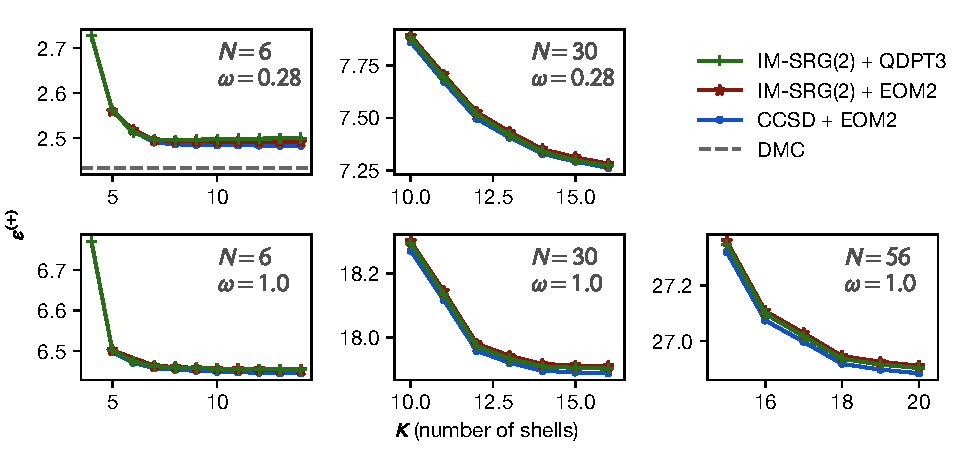
\includegraphics[\textwidth]{EOM/fig-add2.pdf}
  \caption{Progress of ab-initio nuclear structure from calculations of ground-state energies with NN+3N interactions.  Early progress was approximately linear as the problem size scaled with Moore's law while more recent progress has taken advantage of new algorithms which have outpaced Moore's law.  Data taken from \cite{HERGERTPRIVATE}.}
  \label{fig:QDadd}
\end{figure}

\begin{figure}[h]
  \centering
  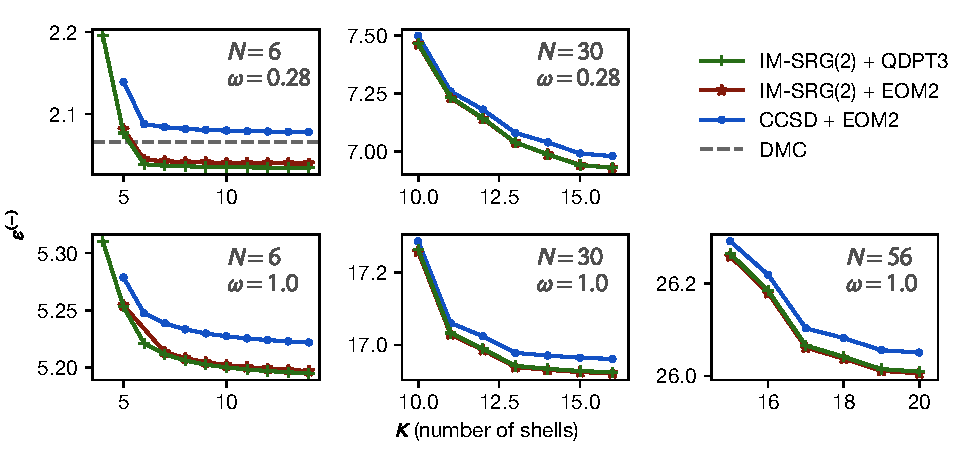
\includegraphics[\textwidth]{EOM/fig-rm2.pdf}
  \caption{Progress of ab-initio nuclear structure from calculations of ground-state energies with NN+3N interactions.  Early progress was approximately linear as the problem size scaled with Moore's law while more recent progress has taken advantage of new algorithms which have outpaced Moore's law.  Data taken from \cite{HERGERTPRIVATE}.}
  \label{fig:QDrm}
\end{figure}

\end{document}
